\chapter{Using the VSDT in ILIas}

% TODO am Ende noch andere Teile voruebergehend auskommentieren, die fuer ILIas
% weniger relevant sind (kommt da ueberhaupt wesentlich was zusammen?)
% - BPEL- und STP-Trafo-Zeugs (oder Trafo-Zeugs allgemein?)
% - JIAC-Node-Plugin?
% - Layout-Algorithmus (kann evtl. generell weg, oder in nen Anhang)

% Intro VSDT in ILIas (von Silvan, aus dem Meilenstein 2)
In order to create processes for managing the smart grid environment, a
corresponding development environment is adopted for better process creation and
-improvement.  One part of this environment is the process oriented development
of services for the SmaGriM system.  The main elements for this are services that
are provided as well defined functionalities by a service provider, in order to
allow service consumers to use those functionalities.  Such services can be
combined into processes that define concrete combinations of service calls, thus
realizing more complex functionalities.  Such processes are also called service
compositions and provide an easy to read yet powerful modeling approach for the
required grid management functionalities.

% Intro Prozess-Simulation (von Silvan, aus dem Meilenstein 2)
The ILIas system allows for extensive testing of services and processes developed
for the SmaGriM platform.  Simulations that are used to predict the behavior of
the grid to specific actions can also be used to test the effects of new or changed
implementations in what-if simulation scenarios.  Such scenarios are realized as
extended test cases by defining a test grid with known behavior, simulating new
services and processes in this scenario and comparing the simulation results to
the expected behavior of the grid.  This allows assessing the effects of changes
in a very concise procedure reducing overall testing efforts.

% Outline dieses Kapitels
Using the Visual Service Design Tool (VSDT), those processes can be modeled,
simulated (tested) using the SmaGriM simulation and finally be deployed to the
system.  In the following Sections, we will describe the general process of using
the VSDT in the ILIas project and then provide details about how to simulate the
process models prior to deploying them to the live system.


%%%%%%%%%%%%%%%%%%%%%%%%%%%%%%%%%%%%%%%%%%%%%%%%%%%%%%%%%%%%%%%%%%%%%%%%%%%%%%%%
%%  The ILIas Development Process                                             %%
%%%%%%%%%%%%%%%%%%%%%%%%%%%%%%%%%%%%%%%%%%%%%%%%%%%%%%%%%%%%%%%%%%%%%%%%%%%%%%%%

\section{The ILIas Development Process}

% TODO Development Process

% verschiedene Rollen und Entwicklungsphasen beschreiben
Several roles can be identified in the ILIas development process.  First, there
is the service provider, developing and providing different basic services to be
orchestrated to complex processes in the process diagram.  Second, there is the
process engineer, creating such orchestrations for handling individual situations,
such as power outages, and deploying them on a repository for later use.  And
finally, there is the SmaGriM maintainer, monitoring the system, whose job is to
select a suitable process from the repository, adapt it to the needs of the
situation, test it in the simulation and finally deploy it to the actual system.

% TODO hier kann man echt mal nen Prozess malen und sich den Text ueber das
% Export-to-Text-Feature erzeugen lassen!

\subsection{The Service Provider}
% Dienst-Provider: Basisdienste bereitstellen

\subsection{The Process Engineer}
% Prozess-Entwickler: Steuerungsprozesse erstellen und in Repository einchecken

\subsection{The SmaGriM Maintainer}
% SmaGriM-Maintainer: Steuerungsprozess aus Repository auschecken, ggf. anpassen,
%     in Simulation durchspielen und auf Produktivsystem deployen


% TODO Prozess anpassen
\begin{figure}
	\centering
	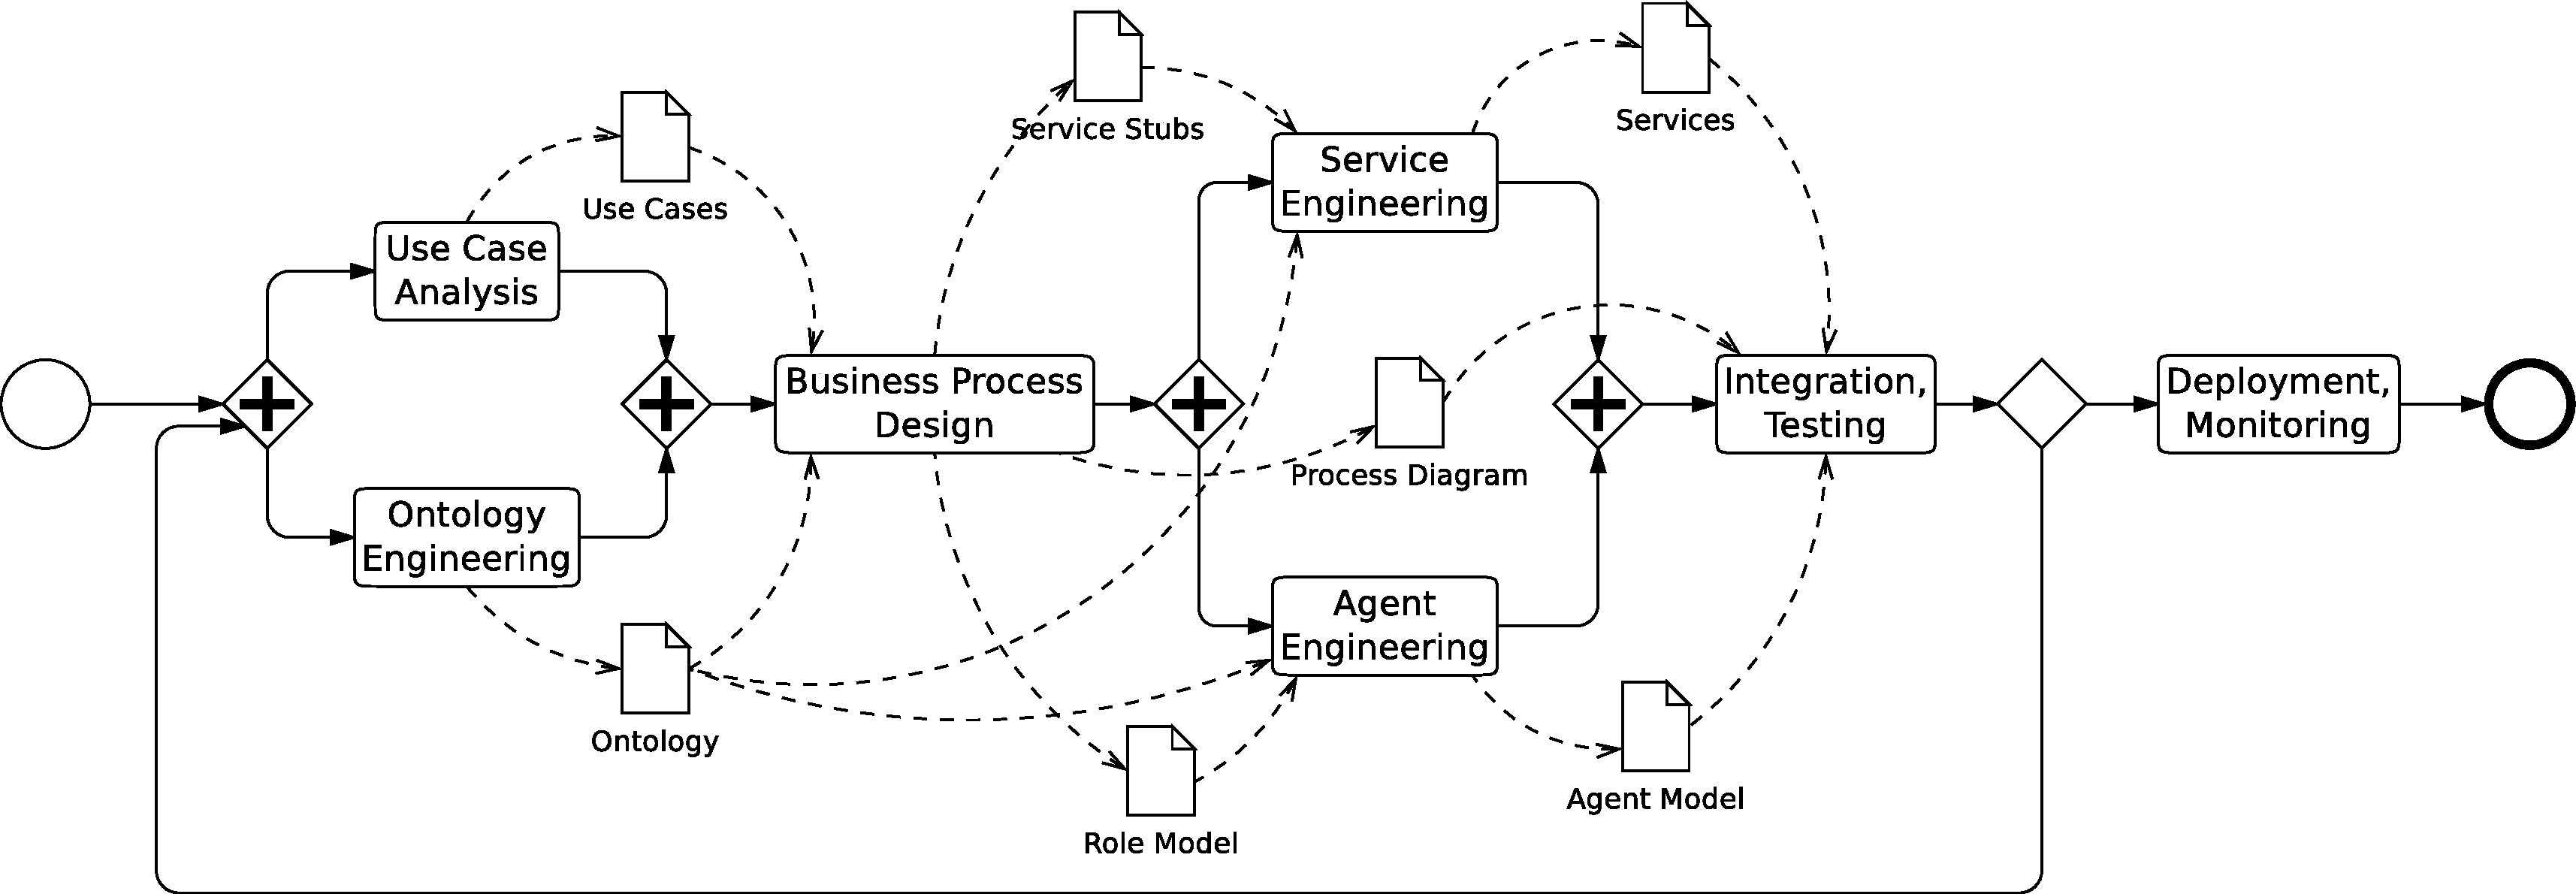
\includegraphics[width=\textwidth]{figures/methodology.pdf}
	\caption{ILIas development process}
	\label{fig:ilias-process}
\end{figure}



%%%%%%%%%%%%%%%%%%%%%%%%%%%%%%%%%%%%%%%%%%%%%%%%%%%%%%%%%%%%%%%%%%%%%%%%%%%%%%%%
%%  Testing Processes in the ILIas Simulation                                 %%
%%%%%%%%%%%%%%%%%%%%%%%%%%%%%%%%%%%%%%%%%%%%%%%%%%%%%%%%%%%%%%%%%%%%%%%%%%%%%%%%

\section{Testing Processes in the ILIas Simulation}

% TODO ILIAS Simulation

\subsection{The ILIas Simulation View}

% Beschreibung des Views
The ILIas Simulation View provides an interface to the ILIas Simulation, where
newly created or adapted process models can be tested for suitability (see
Figure~\ref{fig:ilias-simview}).  The view provides a number of controls for
deploying the process model from the active editor window to the simulation, for
starting and stopping the simulation and for viewing the status of the simulation.

% Funktionsweise: Teil des Node-Plugins, Anbindung an ILIas-Agenten (?)
The Simulation View is based on the \emph{JIAC Node Plugin} (see Section
\ref{sec:user_jiac-node}), and the deployment mechanism is similar to that of the
\emph{Deployment View}, the only difference being that the processes can not be
deployed to arbitrary JIAC agents, but only to to ILIas Simulation Agent.

% Funktionsweise: JADL-Services und Service-Starter-Rules
Like for the regular deployment view, the processes are transformed to executable
JADL services and then deployed to an agent equipped with a JADL interpreter
running on the SmaGriM node.  Additionally, besides the services also a number of
service starter rules are deployed to that agent, so that the individual JADL
services are started just in the way stated by the processes' start events.


% TODO richtiges Bild erstellen und einbinden
\begin{figure}
	\centering
	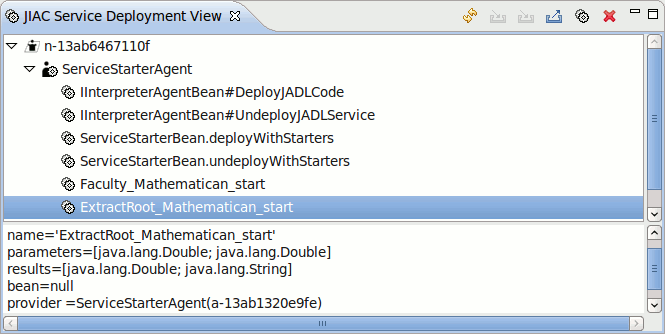
\includegraphics[width=.6\textwidth]{figures/features/deployment-view.png}
	\caption{ILIas Simulation View}
	\label{fig:ilias-simview}
\end{figure}


\subsection{Simulating Processes}
% Klick-Weg zum Simulieren eines Prozesses:
% Welche Bedingungen muessen erfuellt sein, was muss alles eingestellt werden, etc.

% TODO detaillierte Beschreibung

\subsection{Deploying and Executing Processes}
% Nach der Simulation: Deployment auf 'Produktiv-Umgebung' (geht das auch ueber
% die Simulation View, oder verwendet man hierfuer wieder die Deployment View?)




